%% $Id:  $
%% $HeadURL:  $
\documentclass[fleqn]{llncs}

\usepackage{microtype}
\usepackage[utf8]{inputenc}
\usepackage[T1]{fontenc}
\usepackage{amsmath,amssymb}
\usepackage{newtxtext,newtxmath} %\usepackage{times,helvet,courier}

\newcommand{\gringo}{\textit{gringo}}
\newcommand{\clasp}{\textit{clasp}}
\newcommand{\clingo}{\textit{clingo}}
\newcommand{\asprin}{\textit{asprin}}
\newcommand{\asap}{\textit{teaspoon}}
\newcommand{\piclasp}{\textit{piclasp}}

\newcommand{\code}[1]{\lstinline[basicstyle=\ttfamily]{#1}}

\newcommand{\lw}[1]{\smash{\lower1.ex\hbox{#1}}}
\newcommand{\llw}[1]{\smash{\lower3.ex\hbox{#1}}}

%\newcommand{\dataCL}[5]{%
%  \code{#1} & #3 & #5 & #4
%}
%\newcommand{\dataCS}[5]{%
%  #3 & #5 & #4
%}

\newenvironment{tableC}{%
  \scriptsize
  \tabcolsep = 0.6mm
  \begin{tabular}[t]{l|rlr|rlr|rlr|rlr|rlr}\hline
    \multicolumn{1}{l|}{\llw{Instance}} &
    \multicolumn{3}{c|}{UD1} &
    \multicolumn{3}{c|}{UD2} &
    \multicolumn{3}{c|}{UD3} &
    \multicolumn{3}{c|}{UD4} &
    \multicolumn{3}{c}{UD5} \\
    & 
    \multicolumn{1}{c}{Best} & & \multicolumn{1}{c|}{\emph{tea-}} & 
    \multicolumn{1}{c}{Best} & & \multicolumn{1}{c|}{\emph{tea-}} & 
    \multicolumn{1}{c}{Best} & & \multicolumn{1}{c|}{\emph{tea-}} & 
    \multicolumn{1}{c}{Best} & & \multicolumn{1}{c|}{\emph{tea-}} & 
    \multicolumn{1}{c}{Best} & & \multicolumn{1}{c}{\emph{tea-}} \\
    & 
    known & & \emph{spoon} & 
    known & & \emph{spoon} & 
    known & & \emph{spoon} & 
    known & & \emph{spoon} & 
    known & & \emph{spoon} \\
    \hline
  }{%
    \hline
  \end{tabular}
}

\newenvironment{tableB}{%
  \scriptsize
  \tabcolsep = 0.7mm
%  \begin{tabular}[t]{|l|c|r|l|l|l|}\hline
  \begin{tabular}[t]{lcrlll}\hline
    Instance &
    Formulation &
    Time (sec.)\\
    \hline
  }{%
    \hline
  \end{tabular}
}
\newenvironment{tableL}{%
  \scriptsize
  \tabcolsep = 0.7mm
  \begin{tabular}[t]{l|rrrrrrrr|r}\hline
    \lw{Instance} &
    \lw{Time (sec.)} &
    \multicolumn{6}{c}{The best utility vector} &
    The sum of  &
    The best of basic\\
    &
    &
    $(S_1,$ & $S_4,$ & $S_2,$ & $S_7,$ & $S_6,$ & $S_3)$ &
    utility vector &
    and optimized \\
    \hline
  }{%
    \hline
  \end{tabular}
}

%%% Local Variables:
%%% mode: latex
%%% TeX-master: "paper"
%%% End:
 
\newcommand{\paratheory}[2]{\par\emph{{#1}+{#2}:}}
\newcommand{\myparagraph}[1]{\par\textbf{#1}}

% \usepackage{comments} % https://svn.cs.uni-potsdam.de/svn/reposWV/TeXInputs/trunk/comments.sty
% \def\SVNREVISION{$LastChangedRevision: 42 $} % <== is automatically inserted by svn

\usepackage{listings}
\usepackage{pifont}
\newcommand{\cmark}{\ding{51}}%
\newcommand{\xmark}{\ding{55}}%
\usepackage{threeparttable}
\usepackage{booktabs}
\usepackage{tabularx}
\newcolumntype{R}{>{\raggedleft\arraybackslash}X}
%\newcolumntype{R}[1]{>{\raggedleft\arraybackslash}p{#1}}
\usepackage[table]{xcolor}
\usepackage{url}

\lstset{xleftmargin=2\parindent,aboveskip=\smallskipamount,belowskip=\smallskipamount,captionpos=b}
\lstset{numbers=left,numberblanklines=false,basicstyle=\ttfamily}
\lstset{keywords=[1]{m,n},keywordstyle=[1]\usefont{OT1}{cmtt}{m}{n}}

\lstdefinelanguage{clingo}{
  keywordstyle=[1]\usefont{OT1}{cmtt}{m}{n},%
  keywordstyle=[2]\textbf,%
  keywordstyle=[3]\usefont{OT1}{cmtt}{m}{n},%\textit
  alsoletter={\#,\&},%
  keywords=[1]{not,from,import,def,if,else,return,while,break,and,or,for,in,del,and,class},%
  keywords=[2]{\#const,\#show,\#minimize,\#base,\#theory,\#count,\#external,\#program,\#script,\#end,\#heuristic,\#edge,\#project,\#show},%
  keywords=[3]{&,&dom,&sum,&diff,&show},%
  morecomment=[l]{\#\ },%
  morecomment=[l]{\%\ },%
  commentstyle={\color{darkgray}}%
}

\sloppy

\title{\clingo{} goes Linear Constraints over Reals and Integers}

\author{\hspace{-3pt}%
  T. Janhunen\inst{1} % omi
  \and 
  R. Kaminski\inst{3}% oland
  \and
  M. Ostrowski\inst{3}% ax
  \and 
  T. Schaub\inst{2}\inst{3}% orsten
  \and
  S. Schellhorn\inst{3}% ebastian
  \and
  P. Wanko\inst{3}}% hilipp

% \institute{Aalto University \and INRIA Rennes \and Universit\"at Potsdam}
\institute{$^1$Aalto University \quad $^2$INRIA Rennes \quad $^3$University of Potsdam}


\begin{document}

\maketitle

%\begin{abstract}
%	The design space for highly complex system level specifications of embedded systems is enormous as tasks may be mapped to different resources and messages may be routed over several links of the hardware platform. 
%	Furthermore, highly constrained requirements lead to many infeasible solutions that have to be sorted out. \emph{\ac{ASP}} in combination with variant background theories (\emph{\ac{ASPmT}}) has been shown to cope with such requirements very efficiently. However, especially in system level design, a fast \emph{\ac{DSE}} including optimization is crucial in order to steer the development towards optimal design points. In this paper, we therefore propose to couple the highly efficient constraint solving capabilities of \ac{ASP} with a \ac{DSE} including \emph{multi-objective optimization} in an additional background theory. Utilizing the possibility to work on \emph{partial assignments}, \ac{ASPmT} is able to prune entire infeasible and dominated regions from the search space early in the decision process. In the experimental section, we present and compare variant approaches and domain specific heuristics.
%\end{abstract}

\begin{abstract}
	An efficient \emph{\ac{DSE}} is imperative for the design of modern, highly complex embedded systems in order to steer the development towards optimal design points. The early evaluation of design decisions at system-level abstraction layer helps to find promising regions for subsequent development steps in lower abstraction levels by diminishing the complexity of the search problem. In recent works, symbolic techniques, especially \ac{ASPmT}, have been shown to find feasible solutions of highly complex system-level synthesis problems with non-linear constraints very efficiently. In this paper, we present a novel approach to a holistic system-level \ac{DSE} based on \ac{ASPmT}. To this end, we include additional background theories that concurrently guarantee compliance with hard constraints and perform the simultaneous optimization of several design objectives. %First experimental results show the applicability of our approach. %for large optimization of up to 170 tasks mapped to 3-dimensional hardware platforms. Furthermore, it outperforms current multi-objective optimization strategies of \ac{ASP} with respect to both diversity and convergence of found solutions.   %We present and investigate several strategies that show the applicability of our approach even for large problem instances. 
	We implement and compare our approach with a state-of-the-art preference handling framework for \ac{ASP}. Experimental results indicate that our proposed method produces better solutions with respect to both diversity and convergence to the true Pareto front.
\end{abstract}

\section{Introduction}
\label{sec:introduction}
%In order to cope with the ever-increasing complexity of embedded systems, system level description are utilized to diminish the complexity of finding potentially good solutions which can then be used as initial starting points for further optimization in lower abstraction levels. On system level, applications are composed of granular tasks that exchange information over communication messages and form dependency relations between each other. The hardware architecture contains heterogeneous processing elements (e.g.~CPU, DSP, GPU) as well as a communication infrastructure like routers and links. Yet, the design space for such system level specifications of embedded systems is still enormous as tasks may be mapped to different computational resources and messages may be routed over several links of the communication infrastructure.\par 
%Furthermore, various hard constraints like maximum latency and energy consumption of the resulting systems have to be considered. That is, only a subset of all possible decisions leads to valid system implementations that conform to previously defined constraints which makes it even hard\footnote{In fact, the mapping problem is known to be $\mathcal{NP}$-hard \cite{Blickle1998}.} to find \emph{one} feasible solution. However, by encoding the problem symbolically (cf.~\cite{Haubelt2003}) and due to the technological advances in \ac{SAT}, various constraint solvers can be utilized to cope with the complexity. Especially, \emph{\acf{ASP}} has been shown to deal with such stringently constrained design problems very efficiently (e.g.~\cite{Andres2013}). Opposed to other symbolic techniques like \ac{SAT}, reachability can be expressed naturally in \ac{ASP} which fastens the routing sub-problem.\par 
%%\ac{ASP} stems from the area of knowledge representation and reasoning and is based on the \emph{stable model semantics}. 
%Finding one feasible solution is however often insufficient. Depending on the decisions that have been made, the qualitative properties (e.g.~latency, energy consumption, area requirements) of the resulting system implementation may vary considerably from solution to solution. Thus, a \acf{DSE} is imperative to find solutions with optimal properties. Usually, the objectives (i.e.~optimizing the individual properties) of \acp{MOOP} are conflicting with each other and no single optimal solution but a set of \emph{Pareto optimal} solutions exists. A Pareto optimal solution is characterized by the property that it is not dominated by (i.e.~not worse in all objectives than) any other solution. \par%That is, all Pareto optimal solutions are mutually non-dominated.\par 
%Commonly, meta-heuristics like \acp{MOEA} are utilized to solve \acp{MOOP}. They are based on natural processes and work on sets of solutions (populations) concurrently. Each solution is evaluated by a fitness function with respect to the objectives and the best solutions are combined to create novel solutions for subsequent generations. As the initial population is created by a randomized process, finding feasible solutions becomes a problem for stringently constraint environments. Moreover, because the search is generally not executed systematically but based on combining previously found solutions, \acp{MOEA} tend to run into saturation and stop finding novel solutions after an arbitrary number of iterations.\par
%In the paper at hand, we therefore propose an approach that utilizes an exact symbolic encoding for both the constraint solving and the design space exploration. Based on \ac{ASP}, we tightly integrate background theory solvers, known as \ac{ASPmT}, that handle (non-)linear objectives as well as Pareto filtering of found solutions. Furthermore, they are able to work on partial solutions to prune the search space from infeasible and dominated regions of design points early in the decision process. 
%The contribution of this paper is threefold:
%\begin{enumerate}
%	\item We present a universal framework for preference handling that is capable of both linear and non-linear objectives based on \ac{ASPmT}.
%	\item In order to combine various background theories for multi-objective optimization and constraint solving concurrently, we present various approaches.
%	\item Extensive experimental test instances show the advantages and disadvantages of the different approaches. 
%\end{enumerate}\par
%\textbf{Paper organization:} Related work will be covered in Sec.~\ref{sec:relatedwork}. Afterwards, the execution model that will be used throughout the paper is briefly described in Sec.~\ref{sec:model}. Section \ref{sec:framework} contains detailed information about our proposed preference handling framework. Experimental results are given in Sec.~\ref{sec:experiments} before Sec.~\ref{sec:conclusion} concludes the paper.

%Essentially, there are three approaches to explore the design space \cite{Pimentel2017}: First, meta-heuristics like evolutionary algorithms have been studied thoroughly in the past (e.g.~\cite{1,2,3,4,5}). Those techniques are inspired by the natural selection process and work on whole sets of solutions (populations) concurrently. Each solution is evaluated and the best are combined to create new solutions for the following generations. One major problem arises if, due to various hard constraints, only a small subset of design points is feasible. Because of their random nature, pure meta-heuristics tend to fail in finding feasible regions of the design space. \par 
%Therefore, the second approach type combines meta-heuristics with exact methods (e.g.~\cite{Neubauer2016,Haubelt2003,Lukasiewycz2012a}). That is, not the decision variables themselves but the heuristics that are used by the constraint solver are subject to the randomized exploration process. Every found design point is thereby guaranteed to be feasible.\par 
%Finally, exact methods have been developed to explore the design space systematically. While meta-heuristics normally only cover a limited portion of the design space, exact methods (e.g.~\cite{6,7,8,9}) such as \ac{ILP} and branch-and-bound algorithms are guaranteed to find the optimal solutions. \par
%However, the latter are often infeasible for real-world problems as the design space is simply too vast to evaluate every design point.
%However, finding even \emph{one} feasible solution that conforms to all constraints is an $\mathcal{NP}$-hard problem (cf.~\cite{Blickle1998}).
%One way to cope with such complexities is to represent such problems symbolically and utilize specialized solvers like \ac{SAT} (e.g.~\cite{Neubauer2016}), \ac{ILP} (e.g.~\cite{Lukasiewycz2008}), or \acf{ASP} (e.g.~\cite{Andres2013}). 
%In combination with variant background theories, known as \acf{ASPmT}, it is able to handle non-linear constraints like latency and energy calculations (\cite{Andres2015,Neubauer2017}). Bases on \ac{ASP}, the preference handling framework  that is able to compute preferred (optimal) solutions.

%\begin{itemize}
%	\item Partial solutions $\ldots$ dominance checks, infeasibility
%	\item MOEAs three problems: saturation, finding initial solutions, complete solutions
%	\item symbolic encoding
%\end{itemize}>>>>>>> .r56897


In order to cope with the ever-increasing complexity of embedded systems, system-level descriptions are utilized to diminish the complexity of finding potentially good solutions which can then be used as initial starting points for further optimization in lower abstraction levels. At system level, applications are composed of communicating tasks while the hardware architecture contains heterogeneous processing elements (e.g.~CPU, DSP, GPU) as well as a communication infrastructure like routers and links. 
%Yet, the design space for such system-level specifications of embedded systems is still enormous as tasks may be mapped to different computational resources and communication messages may be routed over several links of the communication infrastructure.\par 
%Furthermore, various hard constraints like maximum latency and energy consumption of the resulting systems have to be considered. That is, only a subset of all possible decisions leads to valid system implementations that conform to previously defined constraints which makes it even hard\footnote{In fact, the mapping problem is known to be $\mathcal{NP}$-hard \cite{Blickle1998}.} to find \emph{one} feasible solution. However, by encoding the problem symbolically (cf.~\cite{Haubelt2003}) and due to the technological advances in \ac{SAT}, various constraint solvers can be utilized to cope with the complexity. Especially, \emph{\acf{ASP}} has been shown to deal with such stringently constrained design problems very efficiently (e.g.~\cite{Andres2013}). Opposed to other symbolic techniques like \ac{SAT}, reachability can be expressed naturally in \ac{ASP} which fastens the routing sub-problem.\par 
%\ac{ASP} stems from the area of knowledge representation and reasoning and is based on the \emph{stable model semantics}. 
%Finding one feasible solution is however often insufficient. Depending on the decisions that have been made, the qualitative properties (e.g.~latency, energy consumption, area requirements) of the resulting system implementation may vary considerably from solution to solution. Thus, a \acf{DSE} is imperative to find solutions with optimal properties. Usually, the objectives (i.e.~optimizing the individual properties) of \acp{MOOP} are conflicting with each other and no single optimal solution but a set of \emph{Pareto optimal} solutions exists. A Pareto optimal solution is characterized by the property that it is not dominated by (i.e.~not worse in all objectives than) any other solution. \par%That is, all Pareto optimal solutions are mutually non-dominated.\par 

Depending on the decisions that have been made, the qualitative properties (e.g.~latency, energy consumption, area requirements) of the resulting system implementation may vary considerably from solution to solution resulting into a \ac{MOOP}. Thus, a \acf{DSE} is imperative to find solutions with optimal properties. \par
Essentially, \ac{DSE} approaches can be characterized into two types \cite{Pimentel2017}: First, (meta-)heuristics like evolutionary algorithms and ant colony optimization (e.g.~\cite{Thompson2013,Ferrandi2010}) and second, exact methods such as \ac{ILP} and branch-and-bound algorithms (e.g.~\cite{Lukasiewycz2008,Khalilzad2016}). \par 
Most of the works presented in the field of meta-heuristics extend basic techniques in order to respect domain specific characteristics. For example, in \cite{Thompson2013}, the authors extend genetic algorithms by utilizing domain knowledge. They state, that small differences in design decisions lead to similar system implementations and that symmetrical design points can be pruned. \par 
Another approach (e.g. \cite{Neubauer2016,Schlichter2006}) of handling the infeasibility problem is to integrate dedicated constraint solvers into a \ac{MOEA}. The work of Schlichter et al. \cite{Schlichter2006} integrates, for example, a \ac{SAT} solver into a \ac{MOEA}. Here, the decisions are not directly controlled by the randomized search algorithm of the \ac{MOEA} but the heuristic of the decision variables is subject to exploration. This way, solutions are guaranteed to be feasible.\par
Finally, fully exact methods have been developed to explore the design space systematically. While meta-heuristics normally only cover a limited portion of the design space, exact methods are guaranteed to find the optimal solutions. Nevertheless, for a long time those methods were restricted to single-objective optimization problems only. As one of the few exceptions, Lukasiewycz et al.  \cite{Lukasiewycz2008} present a complete multi-objective Pseudo-Boolean solver based on branch-and-bound algorithms. The results show that this technique is able to find the proven optimal solutions for small problems in a short time. However, exact methods are often replaced in favor of heuristic approaches as the complexity of large systems hinders reasonable employment of those techniques. \par
The disadvantage of using meta-heuristics, on the other hand, is that the initial population is created by a randomized process. Finding feasible regions becomes therefore a problem for stringently constraint environments. Moreover, because the search is generally not executed systematically but based on combining previously found solutions, \acp{MOEA} tend to run into saturation and stop finding novel solutions after a number of iterations.\par
As a remedy, by encoding the problem symbolically, recent advances of constraint solving technologies can be utilized to cope with the complexity of finding feasible solutions. Especially, \emph{\acf{ASP}} has been shown to deal with such stringently constrained design problems very efficiently (e.g.~\cite{Andres2013}). Opposed to other symbolic techniques like \ac{SAT}, reachability can be expressed naturally in \ac{ASP} which fastens the communication synthesis. However, one problem is that non-linear constraints cannot be easily expressed within \ac{ASP}. \par
In the paper at hand, we therefore propose an approach that utilizes an exact symbolic encoding for both constraint solving and design space exploration. To address the shortcomings of \ac{ASP}, we present specific background theory solvers to handle \emph{non-linear objectives} as well as Pareto filtering of found solutions. By utilizing the state-of-the-art \ac{ASP} solver clingo~5 \cite{gekakaosscwa16a}, these background theories can be tightly integrated into the solving process (\emph{\acf{ASPmT}}). This way, we are able to utilize conflict clauses on partial solutions to prune the search space from infeasible and dominated regions of design points early in the decision process. \par
Note that our methodology uses \emph{exact} search strategies with "\emph{any-time}" characteristic, i.e., canceling the search at any time returns an approximate Pareto set that strictly improves with increased solving time until the true Pareto front is reached.\par
%\textbf{Paper organization and contribution:} In the following, we will first reflect upon related work in Sec.~\ref{sec:relatedwork} before the considered specification model and the basics of \ac{ASPmT} are presented in Sec.~\ref{sec:model}. Section \ref{sec:framework} contains the main contribution of the work at hand. Here, we present our proposed universal framework for \acf{DSE} that is capable of multi-objective optimization of both linear and non-linear objectives. For the first time, various approaches for handling the Pareto filtering in a background theory will be presented.    Afterwards, in Sec.~\ref{sec:experiments}, the approaches are evaluated by a number of differently configured test instances. Finally, Sec.~\ref{sec:conclusion} concludes the paper.

%The contribution of this paper is threefold:
%\begin{enumerate}
%	\item We present a universal framework for preference handling that is capable of both linear and non-linear objectives based on \ac{ASPmT}.
%	\item In order to combine various background theories for multi-objective optimization and constraint solving concurrently, we present various approaches.
%	\item Extensive experimental test instances show the advantages and disadvantages of the different approaches. 
%\end{enumerate}\par
%\textbf{Paper organization:} Related work will be covered in Sec.~\ref{sec:relatedwork}. Afterwards, the execution model that will be used throughout the paper is briefly described in Sec.~\ref{sec:model}. Section \ref{sec:framework} contains detailed information about our proposed preference handling framework. Experimental results are given in Sec.~\ref{sec:experiments} before Sec.~\ref{sec:conclusion} concludes the paper.
\section{Curriculum-based Course Timetabling}\label{sec:cb-ctt}

As mentioned, we focus on the curriculum-based course timetabling
(CB-CTT) problems used in the ITC-2007 competition.
The problem description of CB-CTT presented here is based on 
\citep{DBLP:journals/anor/BonuttiCGS12}.

The CB-CTT instance consists mainly of
\textit{curricula},
\textit{courses},
\textit{rooms},
\textit{days}, and
\textit{periods} per day.
A curriculum is a set of courses that shares common students.
We refer to a pair of day and period as \textit{timeslot}.
%
The CB-CTT problem is defined as the task of assigning all lectures
of each course into a weekly timetable, 
subject to a given set of hard and soft constraints.
%
Hard constraints must be strictly satisfied.
Soft constraints are not necessarily satisfied,
but the sum of their violations should be minimal.
%
A \textit{feasible solution} of the problem is an assignment
so that the hard constraints are satisfied.
The objective of the problem is to find a feasible solution with minimal penalty.
%
The CB-CTT problem has the following hard constraints.
\begin{list}{}{}
\item \bm{$H_1$}. \textbf{Lectures}: 
  All lectures of each course must be scheduled, 
  and they must be assigned to distinct timeslots.
\item \bm{$H_2$}. \textbf{Conflicts}: 
  Lectures of courses in the same curriculum or taught by the same
  teacher must be all scheduled in different timeslots.
\item \bm{$H_3$}. \textbf{RoomOccupancy}: 
  Two lectures cannot take place in the same room in the same timeslot.
\item \bm{$H_4$}. \textbf{Availability}: 
  If the teacher of the course is unavailable to teach that course
  at a given timeslot, then no lecture of the course can be scheduled at
  that timeslot.
\end{list}
The CB-CTT problem has the following soft constraints.
\begin{list}{}{}
\item\bm{$S_1$}. \textbf{RoomCapacity}: 
  For each lecture, the number of students that attend the course must
  be less than or equal the number of seats of all the rooms that host
  its lectures. 
  The penalty points, reflecting the number of students above the
  capacity, are imposed on each violation.
\item\bm{$S_2$}. \textbf{MinWorkingDays}: 
  The lectures of each course must be spread into a given minimum
  number of days. 
  The penalty points, reflecting the number of days below the minimum,
  are imposed on each violation.
\item\bm{$S_3$}. \textbf{IsolatedLectures}: 
  Lectures belonging to a curriculum should be adjacent to each other
  in consecutive timeslots. For a given curriculum we account
  for a violation every time there is one lecture not adjacent to any
  other lecture within the same day. 
  Each isolated lecture in a curriculum counts as 1 violation.
\item\bm{$S_4$}. \textbf{Windows}: 
  Lectures belonging to a curriculum should not have time windows
  (periods without teaching) between them. 
  For a given
  curriculum we account for a violation every time there is one
  window between two lectures within the same day. 
  The penalty points, reflecting the length in periods of time window,
  are imposed on each violation.
\item\bm{$S_5$}. \textbf{RoomStability}: 
  All lectures of a course should be given in the same room. 
  The penalty points, reflecting the number of distinct rooms but the first, 
  are imposed on each violation.
\item\bm{$S_6$}. \textbf{StudentMinMaxLoad}: 
  For each curriculum the number of daily lectures should be within a
  given range. 
  The penalty points, reflecting the number of lectures below the minimum or above the
  maximum, are imposed on each violation.
\item\bm{$S_7$}. \textbf{TravelDistance}: 
  Students should have the time to move from one building to another
  one between two lectures. For a given curriculum we account for a
  violation every time there is an \textit{instantaneous move}: 
  two lectures in rooms located in different building in two adjacent
  periods within the same day. 
  Each instantaneous move in a curriculum counts as 1 violation.
\item\bm{$S_8$}. \textbf{RoomSuitability}:
  Some rooms may be not suitable for a given course because of the
  absence of necessary equipment.
  Each lecture of a course in an unsuitable room counts as 1
  violation.
\item\bm{$S_9$}. \textbf{DoubleLectures}:
  Some courses require that lectures in the same day are grouped
  together (\textit{double lectures}). For a course that requires grouped
  lectures, every time there is more than one lecture in one day, 
  a lecture non-grouped to another is not allowed. 
  Two lectures are grouped if they are adjacent and in the same room. 
  Each non-grouped lecture counts as 1 violation.
\end{list}

%%%%%%%%%%%%%%%%%%%%%%%%%%%%%%%%%%%%%%%%%%%%
\begin{table}
\centering
\caption{Problem Formulations}
\label{table:problem_formulations}
%\renewcommand{\arraystretch}{0.9}
%\tabcolsep = 3mm
\begin{tabular}[t]{l|ccccc}\hline
Constraint & UD1 & UD2 & UD3 & UD4 & UD5\\\hline
$H_1$. Lectures &  
H &  H &  H &  H & H\\
$H_2$. Conflicts &  
H &  H &  H &  H & H\\
$H_3$. RoomOccupancy &  
H &  H &  H &  H & H\\
$H_4$. Availability &  
H &  H &  H &  H & H\\
$S_1$. RoomCapacity &  
1 & 1 & 1 & 1  & 1 \\
$S_2$. MinWorkingDays &  
5 &  5 & - & 1 & 5 \\
$S_3$. IsolatedLectures &  
1 & 2 & - & - & 1 \\
$S_4$. Windows &  
- & - & 4 & 1 & 2\\
$S_5$. RoomStability &  
- & 1 & - & - & -\\
$S_6$. StudentMinMaxLoad &  
- & - & 2 & 1 & 2\\
$S_7$. TravelDistance &  
- & - & - & - & 2\\
$S_8$. RoomSuitability &  
- & - & 3 & H & -\\
$S_9$. DoubleLectures &  
- & - & - & 1 & -\\\hline
\end{tabular}
\end{table}
%%%%%%%%%%%%%%%%%%%%%%%%%%%%%%%%%%%%%%%%%%%%

A \textit{formulation} is defined as a specific set of soft constraints
together with the weights associated with each of them.
%
The five formulations UD1--UD5 have been proposed so far.
UD1 is the most basic formulation among them~\citep{DBLP:conf/patat/GasperoS02}.
UD2 is a well known formulation used in the ITC-2007 competition~\citep{GasperoMS/ITC2007}.
UD3, UD4, and UD5 have been recently proposed
to capture more different scenarios~\citep{DBLP:journals/anor/BonuttiCGS12}.
These formulations focus on 
student load (UD3), 
double lectures (UD4), and
travel cost (UD5), respectively.
%
The weights of soft constraints in each formulation is shown in 
Table~\ref{table:problem_formulations}.
The symbol `H' stands for inclusion in a formulation as hard constraint.
The symbol `-' stands for exclusion from a formulation.

In this paper, we formulate the CB-CTT problem as a single-objective
combinatorial optimization problem whose objective function is to
minimize the weighted sum of penalty points in the same manner as
ITC-2007, 
as well as a multi-criteria optimization problem based on lexicographic ordering.
Furthermore, we consider a multi-objective course timetabling problem
combining CB-CTT and Minimal Perturbation Problem.

%%% Local Variables:
%%% mode: latex
%%% TeX-master: "paper"
%%% End:


\section{Multi-Shot ASP Solving with Linear Constraints}
\label{sec:multishot}
Multi-shot solving~\cite{gekakasc14b} is about solving continuously changing logic programs in an operative way.
This can be controlled via reactive procedures that loop on solving while reacting, for instance, to outside changes or previous solving results.
These reactions may entail the addition or retraction of rules that the operative approach can accommodate by leaving the unaffected program parts
intact within the solver.
This avoids re-grounding and benefits from heuristic scores and nogoods learned over time.
%
In fact, 
evolving logic programs with linear constraints can be extremely useful in dynamic applications, for example, to %:
add new resources in a planning domain,
or to set the value of an observed variable measured using sensors.
The abstraction from actual constraints to constraint atoms
allows us to easily extend multi-shot solving to lc-programs.

To illustrate how seamlessly our systems \clingod{dl} and \clingod{lp} support multi-shot solving,
we apply the exemplary \python\ script, shipped with \clingo\ to illustrate incremental solving,
to model the spoiling Yale shooting scenario~\cite{caotpo00a}.
%
Multi-shot solving in \clingo\ relies on two directives (cf.~\cite{gekakasc14b}),
the \texttt{\#program} directive for regrouping rules
and
the \texttt{\#external} directive for declaring atoms
as being external to the program at hand.
The truth value of such external atoms can be set via \clingo's API\@.
The aforementioned \python\ script loops over increasing integers until a stop criterion is met.
It presupposes three groups of rules declared via \texttt{\#program} directives.
At step 0 the programs named \texttt{base} and \texttt{check(n)} are grounded and solved for $\texttt{n}=0$.
Then, in turn programs \texttt{check(n)} and \texttt{step(n)} are added for $\texttt{n}>0$, grounded, and the resulting overall program solved.
% Other names and components are definable by appropriate changes to the script.
% Stop criteria can be the satisfiability or unsatisfiability of the respective program at each iteration.
In addition, at each step $\texttt{n}$ an external atom \texttt{query(n)} is introduced;
it is set to true for the current iteration $\texttt{n}$ and false for all previous instances with smaller integers than $\texttt{n}$.
We refer the reader to~\cite{gekakasc14b} for further details on the \python{} part.
Notably, for dealing with lc-programs,
we can use the exemplary \python\ script as is---once the respective propagator is registered with the solver.

In the spoiled Yale shooting scenario~\cite{caotpo00a},
we have a gun and two actions, viz.\ load and shoot.
If we load, the gun becomes loaded.
If we shoot, it kills the turkey, if the gun was loaded for no more than 35 minutes.
Otherwise, the gun powder is spoiled.
We model this planning problem in \ASPm{lc}.
% --------------------------------------------------------------------------------
\lstinputlisting[caption={Spoiled Yale shooting instance},float=ht,label=encoding:yalebase,basicstyle=\ttfamily\footnotesize]{encodings/base.lps}
% --------------------------------------------------------------------------------
We start by including the incremental \python\ program,
the grammar, and the propagator for linear constraints in the first line of Listing~\ref{encoding:yalebase}.%
\footnote{For uniformity, we use semi-colons '\texttt{;}' rather than '\texttt{,}' for separating body elements.}
This listing is the base program.
All actions and their durations are introduced in Lines~4 and~5.
At the initial situation, the gun is unloaded (Line~6).
Line~7 and~8 initialize integer variables \texttt{at(0)} and \texttt{armed(0)} with 0 (see below).
% --------------------------------------------------------------------------------
\lstinputlisting[caption={Spoiled Yale shooting scenario},float=ht,label=encoding:yale,basicstyle=\ttfamily\footnotesize]{encodings/yale.lps}
% --------------------------------------------------------------------------------
Listing~\ref{encoding:yale} gives the dynamic part of the problem;
it is grounded for each step \texttt{n}.
Line~2 enforces that exactly one action is done per step.
The exact times at which each step takes place is captured by the integer variables \texttt{at(n)}.
The difference between two consecutive time steps is the duration
of the respective action (Line~3).
%
The next three lines make the fluents inertial, viz.\
the gun stays loaded/unloaded if it was loaded/unloaded before,
and the turkey remains dead.
%
Lines~9 and~10 use the integer variable \texttt{armed(n)}
to describe for how long the weapon has been loaded at step \texttt{n}.
Whenever it is unloaded, \texttt{armed(n)} is 0,
otherwise it is increased by the duration of the last action.
%
The following four lines (12--15) encode the conditions and effects of the actions.
When we load the gun, it becomes loaded; when we shoot, it becomes unloaded.
If we shoot and the gun was loaded for no longer than 35 minutes (and thus the gun powder is unspoiled),
the turkey is dead.
The last line ensures that we cannot shoot if the gun is not loaded.
Together with the initial situation and the actions from Listing~\ref{encoding:yalebase}
this encodes the spoiled Yale shooting problem,
and any solution represents an executable plan.
% --------------------------------------------------------------------------------
\lstinputlisting[caption={Query for the spoiled Yale Shooting Scenario.},float=ht,label=encoding:yalequery,basicstyle=\ttfamily\footnotesize]{encodings/query.lps}
% --------------------------------------------------------------------------------
Listing~\ref{encoding:yalequery} adds a query to our problem.
In Line~2 we require that the turkey is dead at step \texttt{n}.
As this constraint is subject to the external atom \texttt{query(n)},
it is only active at solving step \texttt{n}.
The next line ensures that we kill the turkey within 100 minutes.
And as an additional constraint,
we added some preparation time such that we are not allowed 
to shoot in the first 35 minutes.
%
It is possible to solve this problem within three steps.
There exist two solutions at this time point,
one of them containing
\texttt{unloaded(0)}, \texttt{do(wait,1)}, \texttt{unloaded(1)},
\texttt{do(load,2)}, \texttt{loaded(2)},
\texttt{do(shoot,3)}, \texttt{unloaded(3)}, \texttt{dead(3)}.
That is, we simply wait before loading and shooting.
The second solution loads the gun instead of waiting,
thus loading the gun twice before shooting.

%%% Local Variables:
%%% mode: latex
%%% TeX-master: "paper"
%%% End:

\section{Propagator Interface}\label{sec:system}

We now turn to the implementation of theory propagation in \clingo~5
and detail the structure of its interface depicted in Figure~\ref{fig:interface}.
%
\begin{figure}
  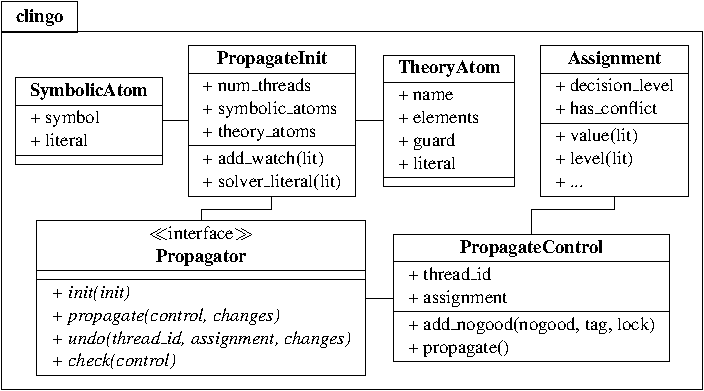
\includegraphics[width=\textwidth]{figures/python-interface}
  \caption{Class diagram of \clingo's (theory) propagator interface\label{fig:interface}}
\end{figure}
%
% To begin with,
The interface \code{Propagator} has to be implemented by each custom propagator.
After registering such a propagator with \clingo,
its functions are called during initialization and search as indicated % in the algorithm
in Figure~\ref{fig:cdcl}.
%
Function \code{Propagator.init}%
\footnote{For brevity, we below drop the qualification \code{Propagator} and use its function names unqualified.}
is called once before solving (Line~(\ref{fig:cdcl:init}) in Figure~\ref{fig:cdcl})
to allow for initializing data structures used during theory propagation.
It is invoked with a \code{PropagateInit} object providing access to symbolic (\code{SymbolicAtom}) as well as theory (\code{TheoryAtom}) atoms.
Both kinds of atoms are associated with program literals,\footnote{Program literals are also used in the \aspif\ format (see~\ref{sec:aspif}).} % ~\cite{gekakaosscwa16b}
which are in turn associated with solver literals.%
\footnote{Note that \clasp's preprocessor might associate a positive or even negative solver literal with multiple atoms.}
Program as well as solver literals are identified by non-zero integers, where positive and negative numbers represent positive or  negative literals, respectively.
In order to get notified about assignment changes, a propagator can set up watches on solver literals during initialization.

During search, function \codeClass{Propagator}{propagate} is called with a \code{PropagateControl} object
and a (non-empty) list of watched literals that got assigned in the recent round of unit propagation (Line~(\ref{fig:cdcl:propagate}) in Figure~\ref{fig:cdcl}).
The \code{PropagateControl} object can be used to inspect the current assignment, record nogoods, and trigger unit propagation.
Furthermore, to support multi-threaded solving,
its \code{thread\_id} property identifies the currently active thread,
each of which can be viewed as an independent instance of the CDCL algorithm in Figure~\ref{fig:cdcl}.%
%Hence, thread-specific state has to be associated with the \code{thread\_id}.
\footnote{%
Depending on the configuration of \clasp, threads can communicate with each other.
For example, some of the recorded nogoods can be shared.
This is transparent from the perspective of theory propagators.}
%
Function \codeClass{Propagator}{undo} is the counterpart of \codeClass{Propagator}{propagate}
and called whenever the solver retracts assignments to watched literals (Line~(\ref{fig:cdcl:undo}) in Figure~\ref{fig:cdcl}).
In addition to the list of watched literals that have been retracted (in chronological order),
it receives the identifier and the assignment of the active thread.
%
Finally, function \codeClass{Propagator}{check} is similar to \codeClass{Propagator}{propagate},
yet invoked without a list of changes.
Instead, it is (only) called on total assignments
(Line~(\ref{fig:cdcl:check}) in Figure~\ref{fig:cdcl}), independently of watches.
%
Overriding the empty default implementations of propagator methods is optional.
% Implementing the propagator methods, which default to empty implementations, is optional. % that does nothing.
For brevity, we below focus on implementations of the methods in \python,
while \lua\ or \C\ could be used as well.

For illustration,
consider Listing~\ref{prg:pigeon:propagator} giving a propagator for (half of) the pigeon-hole problem.
%
\lstinputlisting[linerange={1-10,12-39},float=t,mathescape=true,escapeinside={\#(}{\#)},basicstyle={\ttfamily\small},label={prg:pigeon:propagator},caption={Propagator for the pigeon-hole problem},language=clingo]{example/pigeon-py.lp}
%
Although this setting is constructed, it showcases central aspects
that are also relevant when implementing more complex propagators,
e.g., the \code{Pigeonator} is both stateful and can be used with multiple threads.
%
The underlying ASP encoding is given in Line~\ref{prg:pigeon:prop:rule1}:
A (choice) rule generates solution candidates by placing each of the $p$ pigeons in exactly one among $h$ holes.
While the rule commented out in Line~\ref{prg:pigeon:prop:rule2} would ensure that there is at most one pigeon per hole,
this constraint is handled by the \code{Pigeonator} class
implementing the \code{Propagator} interface (except for \code{check}) in Lines~\ref{prg:pigeon:prop:begin-init}--\ref{prg:pigeon:prop:end-undo}.
Whenever two pigeons are placed in the same hole, it adds a binary nogood forbidding the placement.
To this end,
it maintains data structures for, given a newly placed pigeon,
detecting whether there is a conflict.
%
More precisely, the propagator has two data members:
The \code{self.place} dictionary in Line~\ref{prg:pigeon:prop:member-place} maps solver literals
for \code{place}$/2$ atoms to their corresponding holes,
and the \code{self.state} list in Line~\ref{prg:pigeon:prop:member-state} stores for each solver thread its current placement of pigeons
as a mapping from holes to true solver literals for \code{place}$/2$ atoms.

Function \codeClass{Pigeonator}{init} in Lines~\ref{prg:pigeon:prop:begin-init}--\ref{prg:pigeon:prop:end-init}
sets up watches as well as the dictionaries in \code{self.place} and \code{self.state}.
%
To this end,
it traverses (symbolic) atoms over \code{place}$/2$ in Lines~\ref{prg:pigeon:prop:init:loop-atoms}--\ref{prg:pigeon:prop:init:end-loop-atoms}.
Each such atom is associated with a solver literal, % in \clasp,
obtained in Line~\ref{prg:pigeon:prop:init:map-literal}.
The mapping from the solver literal to its corresponding hole is then stored in the \code{self.place} dictionary in
Line~\ref{prg:pigeon:prop:init:map-lit-hole}.
%
In the last line of the loop, a watch is added for each solver literal at hand,
so that the solver calls \code{propagate} whenever a pigeon is placed. % in the hole as specified by the placement atom.
%
Finally, in Line~\ref{prg:pigeon:prop:init:state}, the \code{self.state} list
of placements per thread,
subject to change upon propagation and backjumping,
% Given a solving thread $i$, each state \code{self.state[$i$]} is a dictionary mapping holes to placement atoms given by their literals.
is initialized with empty dictionaries.

Function \codeClass{Pigeonator}{propagate}, given in Lines~\ref{prg:pigeon:prop:begin-prop}--\ref{prg:pigeon:prop:end-prop},
accesses \code{control.thread\_id} in Line~\ref{prg:pigeon:prop:prop:state}
to obtain the \code{holes} dictionary storing the active thread's current placement of pigeons.
% At first, in Line~\ref{prg:pigeon:prop:prop:state},
% \code{control.thread\_id} is used to obtain the dictionary storing the current thread's partial placement of pigeons.
The loop in Lines~\ref{prg:pigeon:prop:prop:begin-loop}--\ref{prg:pigeon:prop:prop:end-loop} then iterates over the list of changes,
i.e., solver literals representing newly placed pigeons.
After in Line~\ref{prg:pigeon:prop:prop:pigeon-to-hole}
determining the \code{hole} associated with a recently assigned literal,
% , the target \code{hole} associated with the current literal is obtained.
% Then,
\python's \code{setdefault} function is used to update the state:
Depending on whether \code{hole} already appears as a key in the \code{holes} dictionary,
the function either retrieves its associated literal or inserts the new literal under key \code{hole}. % into the dictionary.
While the latter case amounts to updating the placement of pigeons, the former signals a conflict,
triggered by recording a binary nogood in Line~\ref{prg:pigeon:prop:prop:add-clause}.
% In case of a conflict, the propagator adds a binary nogood in Line~\ref{prg:pigeon:prop:prop:add-clause} preventing such an invalid placement of pigeons.
Given that the solver has to resolve the conflict and backjump,
the call to \code{add\_nogood} always yields false, so that
propagation stops without processing remaining changes any further.\footnote{%
  The optional arguments \code{tag} and \code{lock} of \code{add\_nogood} can be used to control the scope and lifetime of recorded nogoods.
  Furthermore, in a propagator that does not add violated nogoods only, % but also unit-resulting nogoods
  function \code{control.propagate} can be invoked to trigger unit propagation.
  }
% Furthermore, using dictionaries \code{state[i]} and \code{place}, conflicts are detected in constant time.

Function \codeClass{Pigeonator}{undo} in Lines~\ref{prg:pigeon:prop:begin-undo}--\ref{prg:pigeon:prop:end-undo} resets a thread's placement of pigeons upon backjumping.
Similar to \codeClass{Pigeonator}{propagate}, % it is called by each solving thread.
the active thread's current placement
is obtained in Line~\ref{prg:pigeon:prop:undo:state},
and changes are traversed in Lines~\ref{prg:pigeon:prop:undo:begin-loop}--\ref{prg:pigeon:prop:undo:del}.
% The function then loops over the set of changes,
% that is, the literals corresponding to pigeons to be removed from the partial placement in Line~\ref{prg:pigeon:prop:undo:del}.
The latter correspond to retracted solver literals,
for which the condition in Line~\ref{prg:pigeon:prop:undo:test} makes sure
that exactly those stored in Line~\ref{prg:pigeon:prop:prop:setdefault} before are cleared,
thus reflecting that the \code{hole} determined in Line~\ref{prg:pigeon:prop:undo:pigeon-to-hole}
is free again.
%%
Finally,
function \code{main} in Lines~\ref{prg:pigeon:prop:begin-main}--\ref{prg:pigeon:prop:end-main} first registers the \code{Pigeonator} propagator in Line~\ref{prg:pigeon:prop:register},
and then initiates grounding and solving with \clingo.

%%% Local Variables:
%%% mode: latex
%%% TeX-master: "paper"
%%% End:

\begin{table}[ht]
\caption{Comparing related applications}
\label{tab:related}
\center\small
\begin{threeparttable}
\begin{tabular}{@{\!\!}l@{\!\!}@{}c@{}@{}c@{}@{\!}c@{\!}@{\!}c@{\!}@{}c@{}@{\!}c@{\!}@{\!}c@{\!}@{\!}c@{\!}@{\!}c@{\!}@{\!}c@{\!}@{\!}c@{\!}}
\toprule
 & \clingo{}     & \clingo{}     & \clingcon{} & \aspartame{} & \inca{} & \ezcsp{} & \ezsmt{} & \mingo{} & \dingo{} & \sysfont{aspmt} & \dlvhex{}\\
 & [\textsc{dl}] & [\textsc{lp}] &             &              &         &          &          &          &          & \sysfont{2smt}  & [\textsc{cp}]\\\midrule
translation  & \xmark{} & \xmark{} & \cmark{}\tnote{1} & \cmark{} & \xmark{} & \xmark{} & \cmark{} & \cmark{} & \cmark{} & \cmark{} & \xmark{} \\
explicit     & \xmark{} & \xmark{} & \cmark{}\tnote{2} & \cmark{} & \cmark{} & \xmark{} & \xmark{} & \xmark{} & \xmark{} & \xmark{} & \xmark{} \\
non-linear   & \xmark{}\tnote{3} & \xmark{} & \cmark{}\tnote{4} & \cmark{}\tnote{4} & \cmark{} & \cmark{} & \cmark{} & \xmark{} & \xmark{}\tnote{3} & \cmark{} & \cmark{} \\
real numbers & \xmark{} & \cmark{} & \xmark{} & \xmark{} & \xmark{} & \cmark{} & \cmark{} & \cmark{}\tnote{5} & \xmark{} & \cmark{} & \xmark{}\\
optimization & \xmark{} & \cmark{}\tnote{6} & \cmark{} & \cmark{} & \cmark{} & \xmark{} & \xmark{} & \xmark{} & \xmark{} & \xmark{} & \cmark{} \\
non-tight    & \cmark{} & \cmark{} & \cmark{} & \cmark{} & \cmark{} & \cmark{} & \xmark{} & \cmark{} & \cmark{} & \xmark{} & \cmark{} 
\end{tabular}
\begin{tablenotes}\footnotesize
\begin{minipage}{0.5\textwidth}
\item[1] Allows for partial problem translations
\item[2] Lazily created
\item[3] Only difference constraints
\end{minipage}%
\begin{minipage}{0.45\textwidth}
\item[4] Translation of distinct into linear constraints
\item[5] Only for variables
\item[6] Optimization relative to stable models
\end{minipage}
\end{tablenotes}
\end{threeparttable}
\end{table}
%%% Local Variables:
%%% mode: latex
%%% TeX-master: "../paper"
%%% End:

\section{Experiments}\label{sec:experiments}
%
\begin{table}[t]
\caption{Comparison of approximation techniques by 
(a) runtime and timeouts,
(b) diversification quality, and
(c) minimum distance}
\small
\parbox{.32\linewidth}{\centering
\begin{tabular}{|l||r|r|}

\hline
Class & \textit{T} & \textit{TO}  \\ 
\hline
\Alabel{3} & \textbf{165} & \textbf{70} \\
\Alabel{3}-\textit{true} & 200 & 113 \\ 
\Alabel{3}-\textit{all} & 202 & 118 \\ 
\Alabel{3}-\textit{rd} & 277 & 280 \\ 
\Alabel{3}-\textit{pg} & 317 & 351\\
\Alabel{3}-\textit{pg-l-rd} & 354 & 442\\
\Alabel{3}-\textit{false} & 351 & 443 \\ 
\Alabel{3}-\textit{pg-l} & 351 & 443\\
\Alabel{2}-\textit{true} & 482 & 618\\
\Alabel{2}-\textit{rd} & 474 & 648\\
\Alabel{1} & 482 & 672\\
\Alabel{2}-\textit{dist-to} & 528 & 689\\
\Alabel{2}-\textit{all} & 515 & 696\\
\Alabel{2}-\textit{false} & 532 & 696\\
\Alabel{2}-\textit{pg} & 542 & 708\\
\Alabel{2}-\textit{dist} & 572 & 773\\
\hline
\end{tabular} 
}
\parbox{.32\linewidth}{\centering
\begin{tabular}{|l||r|r|}

\hline
Class & \textit{S} & \textit{avg}\\ 
\hline
\Alabel{1} & \textbf{15} & 0.13\\
\Alabel{2}-\textit{dist-to} & 14 & 0.14\\ 
\Alabel{2}-\textit{pg} & 13 & \textbf{0.18}\\ 
\Alabel{3}-\textit{pg-l} & 11 & 0.17\\
\Alabel{3}-\textit{pg-l-rd} & 10 & 0.16\\
\Alabel{2}-\textit{all}  & 10 & 0.15\\
\Alabel{2}-\textit{dist} & 8 & 0.07\\ 
\Alabel{2}-\textit{false} & 8 & 0.15\\ 
\Alabel{2}-\textit{true} & 7 & 0.12\\ 
\Alabel{3}-\textit{false} & 6 & 0.16\\ 
\Alabel{2}-\textit{rd} & 5 & 0.12\\ 
\Alabel{3}-\textit{all}  & 5 & 0.08 \\ 
\Alabel{3}-\textit{true} & 4 & 0.08 \\ 
\Alabel{3}-\textit{rd} & 2 & 0.09 \\ 
\Alabel{3}-\textit{pg} & 1 & 0.09\\
%\Alabel{3}-Hdyn & 1 & 0.09\\ 
\Alabel{3} & 0 & 0.06\\

\hline
\end{tabular} 
}
\parbox{.32\linewidth}{\centering
\begin{tabular}{|l||r|r|}

\hline
Class & \textit{S} & \textit{avg}\\ 
\hline
\Alabel{1} & \textbf{15} & 12.25\\
\Alabel{2}-\textit{dist-to} & 13 & 10.38\\
\Alabel{3}-\textit{pg-l-rd } & 13 & 11.82 \\
\Alabel{2}-\textit{dist} & 12 & 5.31\\
\Alabel{3}-\textit{pg-l} & 12 & 11.10\\
\Alabel{2}-\textit{pg} & 10 & \textbf{12.86}\\
\Alabel{2}-\textit{rd} & 9 & 8.77 \\
\Alabel{3}-\textit{all}  & 7 & 3.99 \\ 
\Alabel{3}-\textit{true} & 6 & 4.00 \\ 
\Alabel{3}-\textit{false} & 6 & 7.07 \\ 
\Alabel{2}-\textit{false} & 6 & 6.80\\
\Alabel{2}-\textit{all}  & 4 & 6.98\\
\Alabel{2}-\textit{true} & 3 & 5.31\\
\Alabel{3}-\textit{rd} & 2 & 6.43\\
\Alabel{3} & 2 & 4.28\\
%\Alabel{3}-Hdyn & 1 & 2.90\\ 
\Alabel{3}-\textit{pg} & 0 & 2.79\\
\hline
\end{tabular} 
}
\label{tab:time_comparison_small}
\label{tab:diverse_comparison_small}
\label{tab:min_dist_comparison_small}
\end{table}
%
In this section, we present experiments focusing on the \emph{approximation} techniques of the \asprin\ system for obtaining most dissimilar optimal
solutions. 
%
While \emph{enumeration} and \emph{replication} provide exact results, they need to calculate and store a possibly exponential number of optimal
models or deal with a large search space, respectively.
%
Those techniques are therefore not effective for most practical applications.
%
For Algorithm~\Alabel{2}, we considered the variations \textit{rd}, \textit{pg}, \textit{true}, \textit{false}, and \textit{all} .
%
In \textit{dist}, we issued no timeout for the computation of the partial interpretation, 
while in \textit{dist-to}, we set a timeout for this computation of half the total possible runtime.
%
For Algorithm~\Alabel{3}, we consider the variations that include no extra ASP computation, namely, 
\textit{rd}, \textit{pg}, \textit{true}, \textit{false}, and \textit{all} .
%
We also evaluated a version without any heuristic modification (named simply \Alabel{3}).
%
Furthermore, following \cite{nadel11a}, 
we considered a variation of \textit{pg}, viz.~\textit{pg-l}, 
where the atoms of the selected partial interpretation are given a higher priority, 
and \textit{pg-l-rd}, extending \textit{pg-l} by fixing initially a random sign to all atoms not appearing in the partial interpretation.

We gathered 186 instances from six different classes: \emph{Design Space exploration (DSE)} from~\cite{angeglharesc13a}, \emph{Timetabling (CTT)}
from~\cite{basotainsc13a}, \emph{Crossing minimization} from the ASP competition 2013, \emph{Metabolic network expansion} from \cite{schthi09a},
\emph{Biological network repair} from \cite{geguivscsithve10a} and \emph{Circuit Diagnosis} from~\cite{sidiqqi11a}.
Since we required instances with multiple optimal solutions, we exclusively focused on Pareto optimality. 
DSE and CTT are inherently multi-objective and therefore we could naturally define a Pareto preference for them. 
For the other classes, we turned single-objective into multi-objective optimization problems by distributing their optimization statements.
First, we split the atoms in the optimization statements into four or eight groups evenly. 
We chose for each group the same preference type, either cardinality or subset minimization, and aggregated them by means of Pareto preference.
We calculated optimal solutions regarding these Pareto preferences.
The same was done for CTT and DSE.
An instance was selected if for some Pareto preference ten optimal solutions could be obtained within 600 seconds by \asprin. 
This method generated 816 instances in total. 
We ran the benchmarks on a cluster of Linux machines with dual Xeon E5520 quad-core 2.26 GHz processors and 48 GB RAM. 
We restricted the runtime to 600 seconds and the memory usage to 20 GB RAM.

Since algorithms~\Alabel{1} and \Alabel{2} involve querying programs over preferences, 
we started by evaluating the different query techniques. 
%
For that, we executed \Alabel{1} with query methods \Qlabel{1} to \Qlabel{4} on all selected instances,
stopping after the first $\mathit{solveQuery}$ call was finished.
%
%We achieved that by first calculating an optimal solution and then finding another optimal solution fulfilling the query that the model has to be dissimilar.
The performance of query techniques \Qlabel{2}, \Qlabel{3}, and \Qlabel{4} was similar regarding runtime and only \Qlabel{1} was clearly worse.
We selected \Qlabel{4} for the remaining experiments due to its slightly lower runtime. 
For more detailed tables, we refer to~\cite{roscwa16b}. % \ref{sec:suptables}.

Next, we approximated four most diverse optimal models with methods \Alabel{1} to \Alabel{3}. 
%
We measured runtime and two quality measures.
The first, called diversification quality~\cite{nadel11a},
gives the sum of the Hamming distances among all pairs of solutions normalized to values between zero and one.
The second is the minimum distance among all pairs of solutions of a set in percent.
%
The solution set size of four was chosen because~\cite{shimazu01a} 
claims that three solutions is the optimal amount for a user,
and considering one additional solution provides further insight into the different quality measures. 
%
For all algorithms that do not use heuristics for diversification, 
we instead enabled heuristics preferring a negative sign for the atoms appearing in preference statements. 
This was observed in~\cite{brderosc15b} to improve performance.

Table~\ref{tab:time_comparison_small}(a) provides in column \textit{T} the average runtime and in column \textit{TO} the sum of timeouts. 
The different methods are ordered by the number of timeouts. 
The best results in a column are shown in bold. 
We see that \Alabel{3} is by far the fastest with 70 timeouts, solving 91\% of the instances. 
Heuristic variations of \Alabel{3} perform the best after that. 
Less invasive heuristics achieve similar runtimes with 113-118 timeouts.
More sophisticated heuristics perform worse at 349-443 timeouts.
In a range from 618 to 773 timeouts, non-heuristic methods solve the least instances by a significant margin.
The results are in tune with the nature of the methods. 
Heuristics modifying the solving process for diversity decrease the performance 
in comparison with solving heuristics aimed at performance, 
but not as much as more complex methods involving preferences over optimal models. 

In particular, non-heuristic methods show many timeouts. 
If we tried to analyze the quality of the solutions by assuming worst possible values for the instances that timed out,
the results would be dominated by these instances. 
To avoid that, we calculated a score independent of the runtime.
We considered all possible parings of the different methods. 
For each pair, we compared only instances where both found a solution set.
The method with better quality value for the majority of instances receives a point. 
Finally, we ordered the subsequent tables according to that score. 
 
In Table~\ref{tab:diverse_comparison_small}(b), for each method we see the score in column \textit{S}, and 
the average of the diversification quality (over the instances solved by the method) in column \textit{avg}. 
This way, we can examine the quality a method has achieved compared to other methods, and also the individual average quality.
\Alabel{1} has the best quality with a score of 15, followed by \Alabel{2}-\textit{dist-to}, \Alabel{2}-\textit{pg}, \Alabel{3}-\textit{pg-l} and \Alabel{3}-\textit{pg-l-rd}.
All of those techniques regard the whole previous solution set to calculate the next solution
and guide the solving strictly to diversity.
\Alabel{2}-\textit{pg}, \Alabel{3}-\textit{pg-l} and \Alabel{3}-\textit{pg-l-rd } are also the first, second and third place, respectively, for average diversification quality. 
Next, with scores ranging from 10-7, we see \Alabel{2} methods 
that do not take into account the whole previous set, 
or that were simply unable to find many solutions at all, as in the case of \Alabel{2}-\textit{dist}. 
Finally, we observe that \Alabel{3} variations only regarding the last solution or no previous information 
perform worst in score and average. 
In these cases, the heuristic does not seem to be strong enough to steer the solving to high quality solution sets, 
and \Alabel{3} uses no heuristic or optimization techniques to ensure diverse solutions.

In analogy to Table~\ref{tab:diverse_comparison_small}(b),
Table~\ref{tab:min_dist_comparison_small}(c) provides information for the minimum distance among the solutions. 
%
% The overall grouping of the methods is similar to Table~\ref{tab:diverse_comparison_small}(b). 
%
The best methods considering score and average minimum distance, 
viz.\ \Alabel{1}, \Alabel{2}-\textit{dist-to}, \Alabel{3}-\textit{pg-l-rd}, \Alabel{3}-\textit{pg-l}, \Alabel{2}-\textit{pg}, utilize information from the whole
previous solution set and have strict diversification techniques. 
%\comment{I cut the part about the different behavior of min distance and diversification. The data is not that clear and it saves space. Maybe if we have space left in the end...}

Overall, plain heuristic methods perform better in regards to runtime 
while more complex methods, depending on all previous solutions, lead to better quality. 
%
Furthermore, \Alabel{3}-\textit{pg-l-rd } and \Alabel{3}-\textit{pg-l} provide the best trade-off between performance and quality. 
%
While \Alabel{1}, \Alabel{2}-\textit{dist-to} and \Alabel{2}-\textit{pg} achieve higher quality, they could solve only 18\%, 16\% and 13\% of the instances. 
%
On the other hand, \Alabel{3}-\textit{pg-l-rd } and \Alabel{3}-\textit{pg-l} provide good diversification quality and minimum distance while solving 46\% of the instances. 
%
%\comment{this section is enough for general conclusion: plain heuristic: fast but bad, maxmin: slow but good, more complex heuristic: tradeoff}


%%% Local Variables: 
%%% mode: latex
%%% TeX-master: "paper"
%%% End: 


\section{Discussion}\label{sec:discussion}

Various ways of adding domain-specific information have been explored in the literature.
%
A prominent approach is to implement forms of preferential reasoning
% , like reasoning wrt inclusion-minimal models, 
by directing choices through
a given partial order on literals~\cite{cacacale96a,rogima10a,giumar12a}.
%
To some degree, this can be simulated by heuristic modifiers like
\hpre{a}{\texttt{false}}{1}
that allow for computing a (single) inclusion-minimal model.
However, as detailed in \cite{rogima10a}, enumerating all such models needs additional constraints
or downstream tester programs.
Similarly,
\cite{balduccini11b} modifies the heuristic of the ASP solver \textit{smodels} to accommodate learning from smaller instances.
See also~\cite{falepf01a,falemari07a}.
Most notably,
\cite{rintanen12a} achieves impressive results in planning by equipping a SAT solver with
planning-specific heuristics.
%
All aforementioned approaches need customized changes to solver implementations.
%
Hence, it will be interesting to investigate how these approaches can be expressed and combined in
our declarative framework.
%
Declarative approaches to incorporating control knowledge can be found in heuristic planning.
For instance, \cite{backab00a} harness temporal logic formulas, while \cite{sierra04a} also uses
dedicated predicates for controlling backtracking in a forward planner.
%
However,
care must be taken when it comes to modifying a solver's heuristics.
Although it may lead to great improvements, it may just as well lead to a degradation of search.
In fact, the restriction of choice variables may result in exponentially larger search spaces~\cite{jajuni05a}.
This issue is reflected in our choice of heuristic modifiers, 
ranging from an \texttt{init}ial bias,
over a continued yet scalable one by \texttt{factor},
to a strict preference with \texttt{level}.

To sum up,
we introduced a declarative framework for incorporating domain-specific heuristics into ASP solving.
The seamless integration into ASP's input language provides us with a general and flexible tool for
expressing domain-specific heuristics.
As such, we believe it to be the first of its kind.
Our heuristic framework offers completely new possibilities of applying, experimenting, and studying
domain-specific heuristics in a uniform setting.
Our example heuristics merely provide first indications on the prospect of our approach,
but much more systematic empirical studies are needed to exploit its full power.


%%% Local Variables: 
%%% mode: latex
%%% TeX-master: "paper"
%%% End: 


\bibliographystyle{splncs} % {plain} % {named}
%\bibliography{lit,procs,akku,own} % https://svn.cs.uni-potsdam.de/svn/reposWV/Papers/bibfiles/trunk
\begin{thebibliography}{10}

% \bibitem{Acuna2009}
% V.~Acu{\~{n}}a, F.~Chierichetti, V.~Lacroix, A.~Marchetti-Spaccamela, M.~Sagot, L.~Stougie.
% \newblock {Modes and cuts in metabolic networks: Complexity and algorithms}.
% \newblock {\em Biosystems}, 95(1):51--60, 2009.

\bibitem{anbole13a}
C.~Ans{\'o}tegui, M.~Bonet, J.~Levy.
\newblock {SAT}-based {MaxSAT} algorithms.
\newblock {\em Artificial Intelligence}, 196:77--105, 2013.

\bibitem{baral02a}
C.~Baral.
\newblock {\em Knowledge Representation, Reasoning and Declarative Problem Solving}.
\newblock Cambridge, 2003.

\bibitem{Becker2007}
S.~Becker, A.~Feist, M.~Mo, G.~Hannum, B.~Palsson, M.~Herrgard.
\newblock {Quantitative Prediction of Cellular Metabolism with Constraint-based Models: The COBRA Toolbox}.
\newblock {\em Nature Protocols}, 2(3):727--738, 2007.

\bibitem{coevgeprscsith13a}
G.~Collet, D.~Eveillard, M.~Gebser, S.~Prigent, T.~Schaub, A.~Siegel, S.~Thiele.
\newblock Extending the metabolic network of {E}ctocarpus siliculosus using answer set programming.
\newblock 
% In P.~Cabalar and T.~Son, editors, {\em Proceedings of the Twelfth International Conference on Logic Programming and Nonmonotonic Reasoning (LPNMR'13)}, volume 8148 of {\em Lecture Notes in Artificial Intelligence}, 
{\em Proceedings LPNMR},
245--256. Springer, 2013.

\bibitem{dantzig63a}
G.~Dantzig.
\newblock {\em Linear Programming and Extensions}.
\newblock Princeton, 1963.

% \bibitem{ebhahe04a}
% O.~Ebenhöh, T.~Handorf, R.~Heinrich.
% \newblock Structural analysis of expanding metabolic networks.
% \newblock {\em Genome Informatics}, 15(1):35--45, 2004.

\bibitem{Ebrahim2013}
A.~Ebrahim, J.~Lerman, B.~Palsson, D.~Hyduke.
\newblock {COBRApy: COnstraints-Based Reconstruction and Analysis for Python.}
\newblock {\em BMC Systems Biology}, 7:74, aug 2013.

\bibitem{gekakaosscwa16a}
M.~Gebser, R.~Kaminski, B.~Kaufmann, M.~Ostrowski, T.~Schaub, P.~Wanko.
\newblock Theory solving made easy with clingo~5.
\newblock 
% In M.~Carro and A.~King, editors, {\em Technical Communications of the Thirty-second International Conference on Logic Programming (ICLP'16)}, volume~52, 
{\em Technical Comm.\ ICLP},
2:1--2:15. 
% Open Access Series in Informatics
OASIcs, 2016.

\bibitem{gekakarosc15a}
M.~Gebser, R.~Kaminski, B.~Kaufmann, J.~Romero, T.~Schaub.
\newblock Progress in clasp series 3.
\newblock 
% In F.~Calimeri, G.~Ianni, and M.~Truszczy{\'n}ski, editors, {\em Proceedings of the Thirteenth International Conference on Logic Programming and Nonmonotonic Reasoning (LPNMR'15)}, volume 9345 of {\em Lecture Notes in Artificial Intelligence}, 
{\em Proceedings LPNMR},
368--383. Springer, 2015.

\bibitem{gellif91a}
M.~Gelfond, V.~Lifschitz.
\newblock Classical negation in logic programs and disjunctive databases.
\newblock {\em New Generation Computing}, 9:365--385, 1991.

\bibitem{haebhe05a}
T.~Handorf, O.~Ebenhöh, R.~Heinrich.
\newblock Expanding metabolic networks: Scopes of compounds, robustness, and evolution.
\newblock {\em J.\ of Molec.\ Evolution}, 61(4):498--512, 2005.

\bibitem{laten2014a}
M.~Latendresse.
\newblock Efficiently gap-filling reaction networks.
\newblock {\em BMC bioinformatics}, 15(1):225, 2014.

\bibitem{marzom16a}
C.~Maranas, A.~Zomorrodi.
\newblock {\em Optimiz.\ methods in metabolic networks}.
\newblock Wiley, 2016.

\bibitem{Orth2010}
J.~Orth, B.~Palsson.
\newblock {Systematizing the generation of missing metabolic knowledge.}
\newblock {\em Biotechnology and bioengineering}, 107(3):403--12, oct 2010.

% \bibitem{orthpa10a}
% J.~Orth, I.~Thiele, B.~Palsson.
% \newblock What is flux balance analysis?
% \newblock {\em Nature biotechnology}, 28(3):245--248, 2010.

\bibitem{ostsch12a}
M.~Ostrowski, T.~Schaub.
\newblock {ASP} modulo {CSP}: The clingcon system.
\newblock {\em Theory and Practice of Logic Programming}, 12(4-5):485--503, 2012.

% \bibitem{potassco}
% Potassco website.
% \newblock http://potassco.org.

\bibitem{prcodideetdaevthcabosito14a}
S.~Prigent, G.~Collet, S.~Dittami, L.~Delage, F.~{Ethis de Corny}, O.~Dameron, D.~Eveillard, S.~Thiele, J.~Cambefort, C.~Boyen, A.~Siegel, T.~Tonon.
\newblock The genome-scale metabolic network of ectocarpus siliculosus (ectogem): a resource to study brown algal physiology and beyond.
\newblock {\em The Plant Journal}, 80(2):367–381, 2014.

\bibitem{Prigent2017}
S.~Prigent, C~.Frioux, S.~Dittami, S.~Thiele, A.~Larhlimi, G.~Collet, F.~Gutknecht, J.~Got, D.~Eveillard, J.~Bourdon, F.~Plewniak, T.~Tonon, A.~Siegel.
\newblock {Meneco, a Topology-Based Gap-Filling Tool Applicable to Degraded Genome-Wide Metabolic Networks}.
\newblock {\em PLOS Computational Biology}, 13(1):e1005276, jan 2017.

\bibitem{Reed2003}
J.~Reed, T.~Vo, C.~Schilling, B.~Palsson.
\newblock {An expanded genome-scale model of Escherichia coli K-12 (iJR904 GSM/GPR).}
\newblock {\em Genome Biology}, 4(9):R54, 2003.

\bibitem{SatishKumar2007}
V.~{Satish Kumar}, M.~Dasika, C.~Maranas.
\newblock {Optimization based automated curation of metabolic reconstructions}.
\newblock {\em BMC Bioinformatics}, 8(1):212, 2007.

\bibitem{schthi09a}
T.~Schaub, S.~Thiele.
\newblock Metabolic network expansion with {ASP}.
\newblock
% In P.~Hill and D.~Warren, editors, {\em Proceedings of the Twenty-fifth International Conference on Logic Programming (ICLP'09)}, volume 5649 of {\em Lecture Notes in Computer Science}, 
{\em Proceedings ICLP},
312--326. Springer, 2009.

\bibitem{siniso02a}
P.~Simons, I.~Niemelä, T.~Soininen.
\newblock Extending and implementing the stable model semantics.
\newblock {\em Artificial Intelligence}, 138(1-2):181--234, 2002.

\bibitem{Thiele2014}
I.~Thiele, N.~Vlassis, R.~Fleming.
\newblock {fastGapFill: efficient gap filling in metabolic networks.}
\newblock {\em Bioinformatics}, 30(17):2529--2531, sep 2014.

\bibitem{Vitkin2012}
E.~Vitkin, T.~Shlomi.
\newblock {MIRAGE: a functional genomics-based approach for metabolic network model reconstruction and its application to cyanobacteria networks.}
\newblock {\em Genome Biology}, 13(11):R111, 2012.

\end{thebibliography}

%%% Local Variables:
%%% mode: latex
%%% TeX-master: "paper"
%%% End:

\end{document}

%%% Local Variables:
%%% mode: latex
%%% TeX-master: t
%%% End:
